\documentclass[10pt,a4paper]{article}
\usepackage[margin=22mm]{geometry}\usepackage[T1]{fontenc}\usepackage{lmodern,microtype,booktabs,graphicx,xcolor,hyperref,tcolorbox,parskip}
\definecolor{ink}{HTML}{172B4D}\definecolor{teal}{HTML}{137C8B}\definecolor{mist}{HTML}{F1F6F8}
\hypersetup{colorlinks=true,linkcolor=teal,urlcolor=teal}
\title{\vspace{-2em}\color{ink}\bfseries IDM-Viz reference and calibrator uncertainty\\[-.2em]\large Block-bootstrap sensitivity on NOAA GSOD}
\author{Phase 3 natural-stream addendum}\date{17 November 2026}
\begin{document}\maketitle\vspace{-1em}
\begin{tcolorbox}[colback=mist,colframe=teal,boxrule=0pt,leftrule=2mm]\textbf{Scope.} One Offutt station, one chronological same-day classification holdout. These bootstrap intervals are conditional sensitivity summaries, not station-population confidence guarantees.
\end{tcolorbox}
\section*{Protocol}
We held the logistic classifier and its training fit fixed, then performed 200 noncircular 30-day moving-block resamples for each of three components: refit the isotonic correctness calibrator only; resample fixed-reference correctness only; and refit/resample both. Each draw yields the 21 batch accuracy estimates and plug-in Poisson-binomial expected-harm concern scores using the same frozen predictions. Monitoring labels are used only to compare estimates with realized accuracy after scoring. No threshold or method is selected from these results. This design isolates uncertainty due to the calibration and reference partitions; it omits model-training uncertainty and does not create independent temporal replications.
\section*{Results}
With the joint bootstrap, mean per-batch 95\% bootstrap interval width for estimated accuracy was 0.045{}; mean interval width for expected-harm concern was 0.219{}. Across the 21 batches, the bootstrap concern decision disagreed with the original plug-in decision in 0.007{} of batch-draws on average. The mean bootstrap standard deviation of reference accuracy was 0.0147{}. These values describe sensitivity to historical calibration/reference sampling under the chosen 30-day block scheme. They do not repair the original stream's weak empirical plug-in interval coverage and must not be generalized beyond this record.
\begin{center}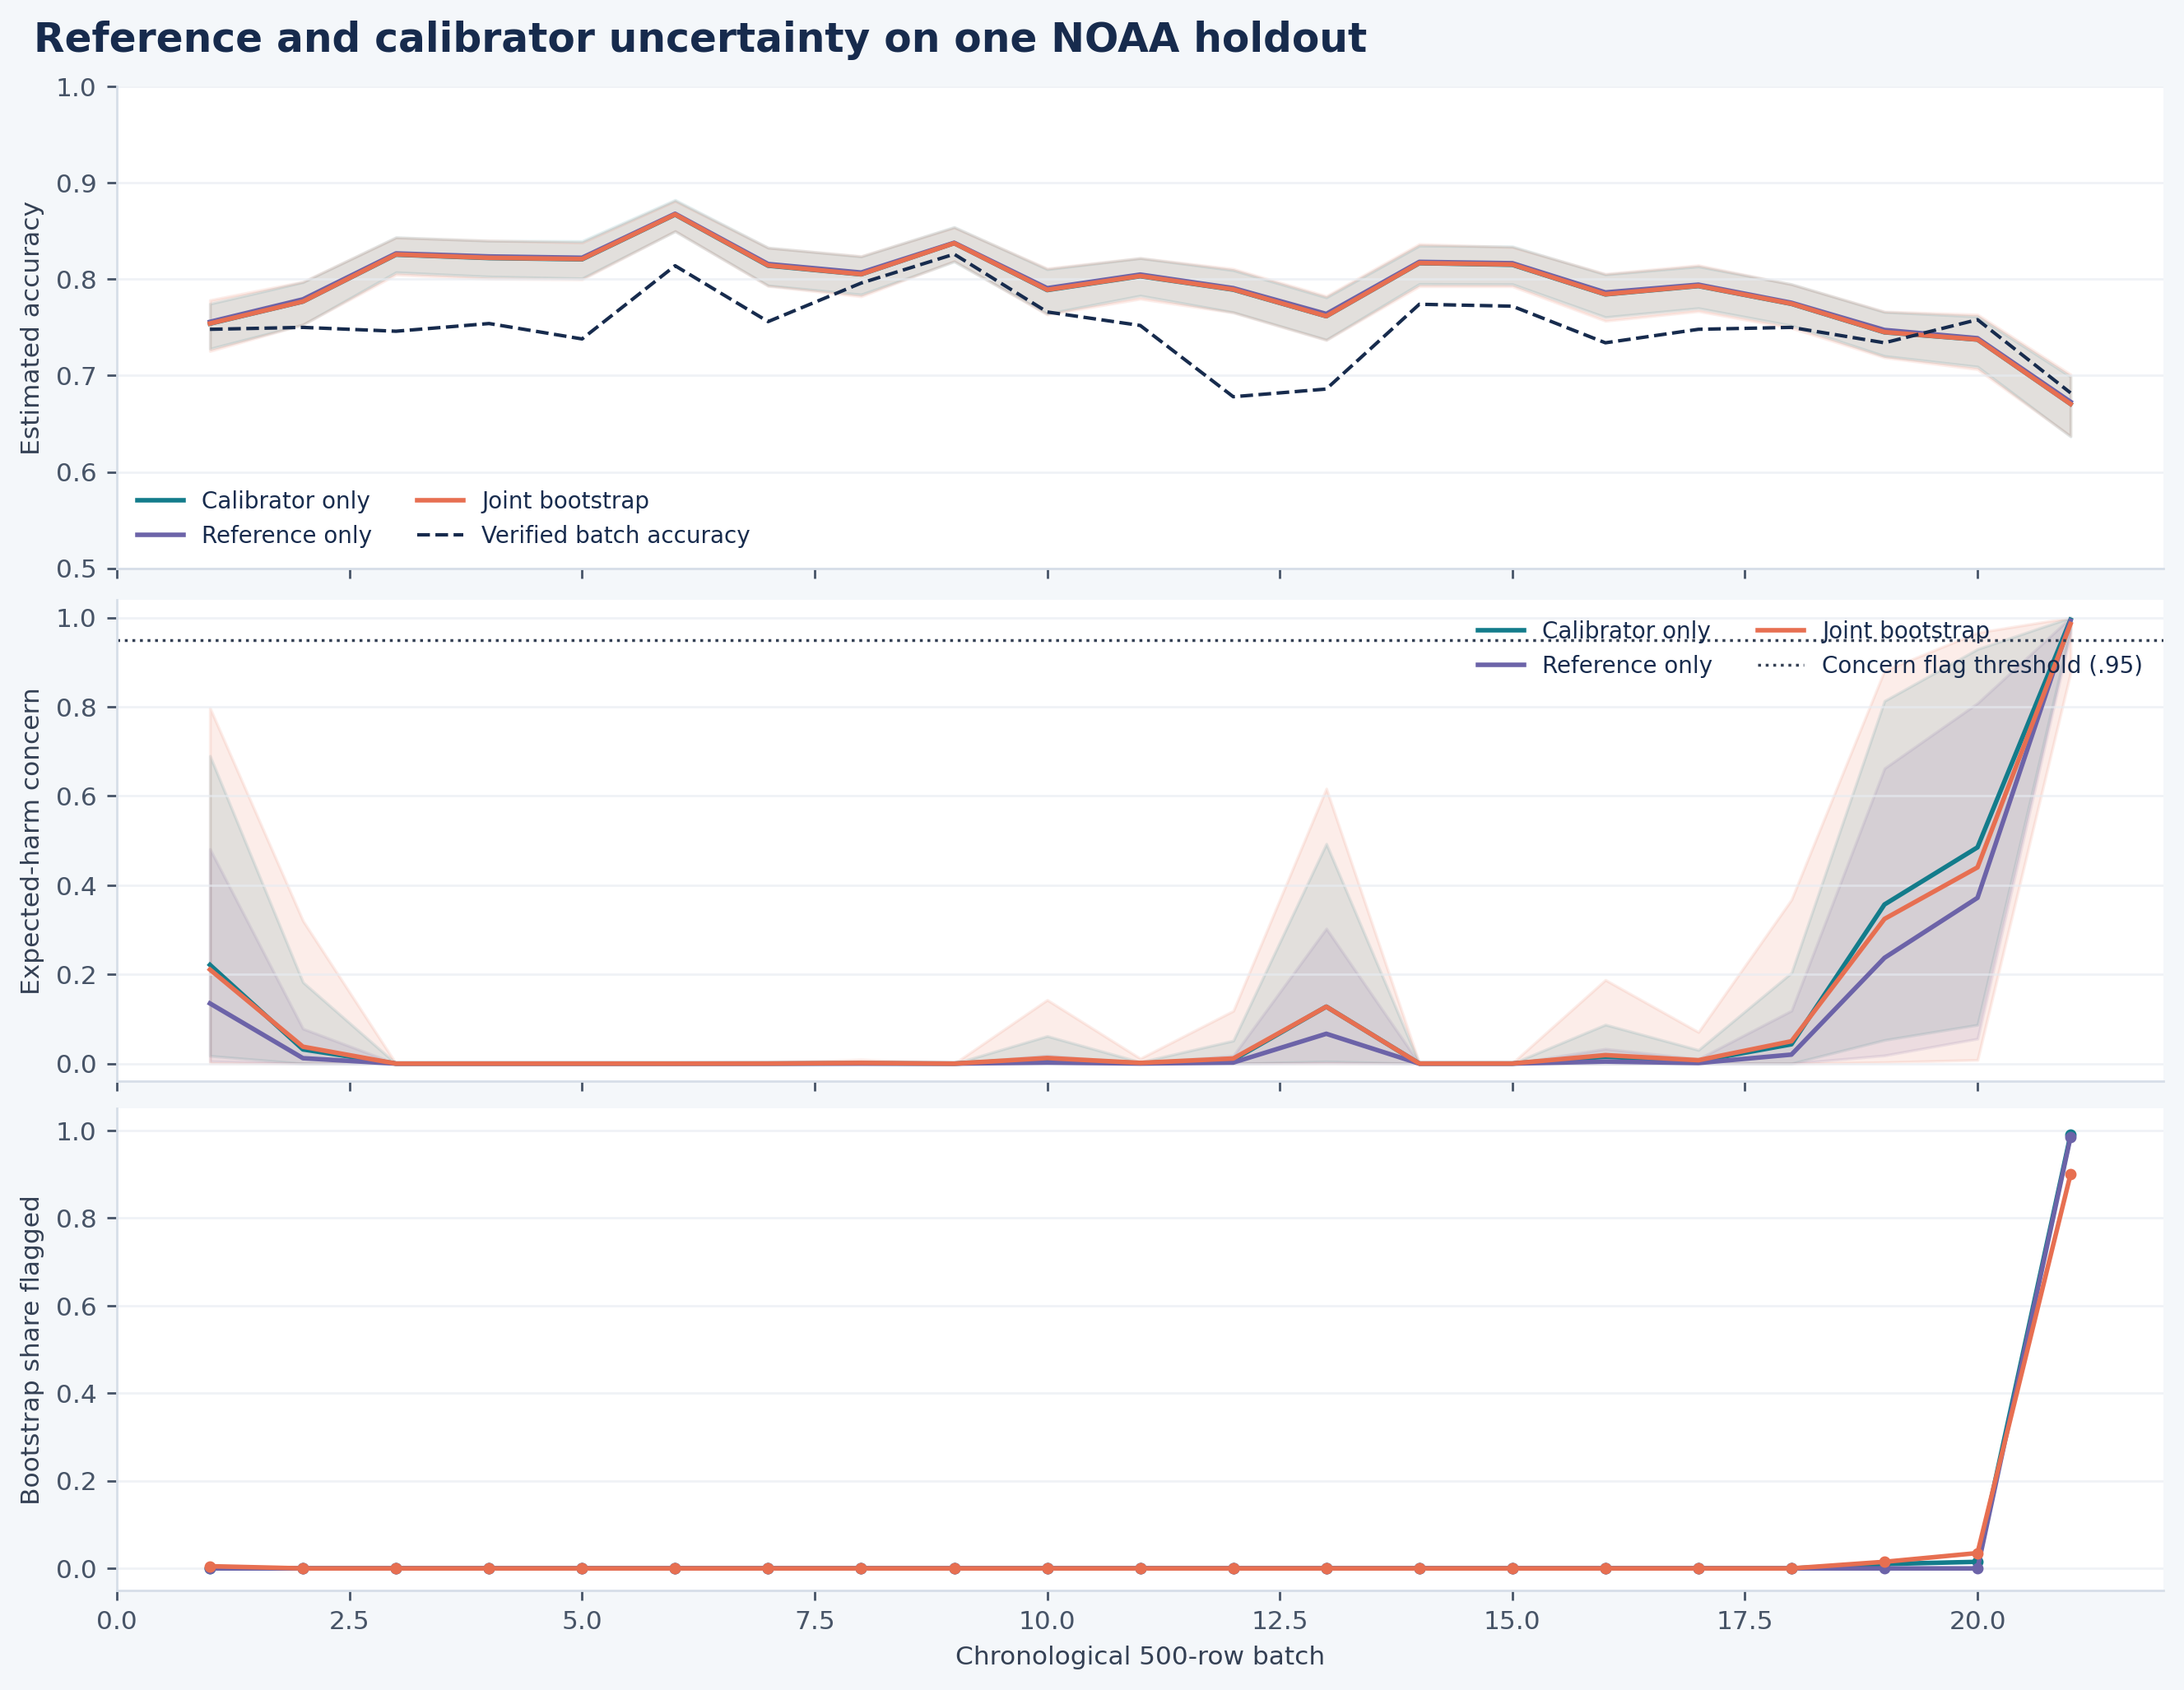
\includegraphics[width=\linewidth]{noaa_uncertainty.png}\end{center}
\section*{Interpretation and limits}
The component comparison separates calibrator variation from reference-accuracy variation and shows where the concern score is unstable. Reference-only resampling leaves the point accuracy estimate unchanged by construction, but can move the expected-harm concern because its benchmark changes. Isotonic refits affect the estimated correctness probabilities. The classifier itself is not refit; station-year autocorrelation may extend beyond 30 days; finite bootstrap replicates add Monte Carlo error; and only one station and one split are available. Consequently these are conditional uncertainty diagnostics, not calibrated guarantees or evidence of natural-domain transfer.
\section*{Reproduction}
\texttt{python scripts/run\_noaa\_reference\_calibration\_uncertainty.py}\\
\texttt{python scripts/summarize\_noaa\_reference\_calibration\_uncertainty.py}\\
Compile this source with Tectonic. Full-precision draws, summaries, source hashes, and software versions are included with the report.
\end{document}
